%-----------------------------------------------------------------------
\documentclass[11pt]{article}
%-----------------------------------------------------------------------
%%%\usepackage{amsfonts,amsmath,amsthm}
%%%\usepackage{algorithm2e,framed,algorithmic}
%%%\usepackage{enumerate,bm}
%%%\input{newcmds}
%%%\input{macros_short.tex}
%-----------------------------------------------------------------------
\addtolength{\textwidth}{1.4in}
\addtolength{\oddsidemargin}{-0.5in}
\addtolength{\evensidemargin}{-0.5in}
%\addtolength{\topmargin}{-0.5in}
\addtolength{\topmargin}{-1.0in}
\addtolength{\textheight}{1.7in}
\newlength{\defbaselineskip}
\setlength{\defbaselineskip}{\baselineskip}

\usepackage{algorithm}
\usepackage{algpseudocode}
\usepackage{framed}
\usepackage{amssymb}
\usepackage{amsfonts}
\usepackage{amsmath}
%%% \usepackage{verbatim}
\usepackage{graphicx}
%\usepackage{caption}
%%\DeclareCaptionType{copyrightbox}
%\usepackage{subcaption}
\usepackage{url}
\usepackage{rotating}
\usepackage{multirow}
\usepackage{color}
\usepackage{xcolor}
%%\usepackage{enumitem}
\usepackage{paralist}

%\usepackage{subfig}
\usepackage{subfigure}

\usepackage{longtable} 
\usepackage{makecell}

%\usepackage[multiple]{footmisc}

%% \addtolength{\textwidth}{1.5in}
%% \addtolength{\oddsidemargin}{-0.75in}
%% \addtolength{\evensidemargin}{-0.75in}
%% %\addtolength{\topmargin}{-0.25in}
%% \addtolength{\topmargin}{-0.5in}
%% %\addtolength{\topmargin}{-1.0in}
%% \addtolength{\textheight}{1.25in}
\definecolor{darkgreen}{rgb}{0,0.6,0}

\usepackage[multiple]{footmisc}
\usepackage[section]{placeins}

\usepackage{hyperref}
\hypersetup{
     colorlinks   = true,
     linkcolor    = blue,
     citecolor    = green
}


%-----------------------------------------------------------------------

%\newlength{\defbaselineskip}
%\setlength{\defbaselineskip}{\baselineskip}
%
\newtheorem{definition}{Definition}
\newtheorem{lemma}{Lemma}
\newtheorem{theorem}{Theorem}
\newtheorem{corollary}{Corollary}

\newtheorem{observation}{Observation}
\newtheorem{claim}{Claim}
\newtheorem{conclusion}{Conclusion}

%% \newenvironment{proof}{\noindent {\em Proof:}}{\\\hspace*{\fill}\mbox{$\diamond$}}
%% \newcommand{\argmin}{\text{argmin}}

\newcommand{\fix}[1]{\textcolor{red}{#1}}
\newcommand{\comment}[1]{\textcolor{blue}{#1}}
\newcommand{\awk}[1]{\textcolor{darkgreen}{#1}}

\newcommand{\argmin}{\text{argmin}}
\newcommand{\Probab}[1]{\mbox{}{\bf{Pr}}\left[#1\right]}
\newcommand{\Expect}[1]{\mbox{}{\bf{E}}\left[#1\right]}
\newcommand{\ExpectBracket}[1]{\mbox{}\langle#1\rangle}

% Here are two macros for comments.
\newcommand {\nred}[1]{{\color{red}\sf{[#1]}}}
\newcommand {\michael}[1]{{\color{red}\sf{[michael: #1]}}}
\newcommand {\charles}[1]{{\color{blue}\sf{[charles: #1]}}}
\newcommand {\charlesX}[1]{{\color{violet}\sf{[charlesG: #1]}}}

\usepackage[normalem]{ulem}


%-----------------------------------------------------------------------
\begin{document}


\title{%
(((
ORIG: 
A Surprising Power Law Relationship Predicts Trends in the Test Accuracy for Very Deep Neural Networks
\\ OR ))) \\ 
Heavy-Tailed Universality Predicts Trends in Test Accuracies for Very Large Pre-Trained Deep Neural Networks
}

\author{%
Charles H. Martin\thanks{Calculation Consulting, 8 Locksley Ave, 6B, San Francisco, CA 94122, \texttt{charles@CalculationConsulting.com}.} 
\and 
Michael W. Mahoney\thanks{ICSI and Department of Statistics, University of California at Berkeley, Berkeley, CA 94720, \texttt{mmahoney@stat.berkeley.edu}.}
}


\date{}
\maketitle

%{\bf
%%   \vspace{5mm}
%   \emph{
%      \begin{center}
%         Note:  This is still a rough draft - from \today. \\
%         Please do NOT distribute.
%      \end{center}
%   }
%%   \vspace{5mm}
%}


\begin{abstract}
\noindent
Given two or more Deep Neural Networks (DNNs) with the same or similar architectures, and trained on the same dataset, but trained with different solvers, parameters, hyper-parameters, regularization, etc., can we predict which DNN will have the best test accuracy, and can we do so without peeking at the test data?   
In this paper, we show how to use our new Theory of Heavy-Tailed Self-Regularization (HT-SR) to answer this. 
The HT-SR theory suggests, among other things,  that modern DNNs exhibit a mechanistic form of Heavy Tailed Universality
in that the correlations in the layer weight matrices can be fit to a power law with exponents that lie in common Heavy Tailed Universality classes from Random Matrix Theory (RMT).
From this, here, we develop a Universal capacity control metric that is a weighted average of these heavy tailed power law exponents, 
Rather than considering small toy NNs, we examine over 50 different, large-scale pre-trained DNNs, ranging over 15 different architectures, trained on 
ImagetNet, each of which has been reported to have different test accuracies. 
We show that this new capacity metrics correlates very well with the reported test accuracies of these DNNs, looking across each architecture (VGG16/.../VGG19, 
ResNet10/.../ResNet152, etc.).
Moreover, we show how to approximate the metric by the more familiar Product Norm capacity measure, as the average of the log  Frobenius norm of the layer weight matrices.
Our approach requires no changes to the underlying DNN or its loss function, it does not require us to train a model (although it could be used to monitor training), and it does not even require access to the ImageNet data.
\end{abstract}



%\vspace{-4mm}

\section{Introduction}
\label{sxn:intro}

Given two or more Deep Neural Networks (DNNs) with the same or similar architectures, and trained on the same dataset, but trained with different solvers, parameters, hyper-parameters, regularization, etc., can we predict which DNN will have the best test accuracy, and can we do so without peeking at the test data?   

\nred{Lead in here could be more engaging}
Solving this question of generalization would have both theoretical impact and great practical importance. 
With respect to the former, solving this would help to understand why this class of machine learning (ML) models performs as well as it does in certain classes of applications.
With respect to the latter, there are many motivating examples.
% 
Here are several.
\begin{itemize}
\item
\textbf{Automating architecture search.}
Developing DNN models often requires significant architecture engineering, so there is interest in automating the design of DNN models, such as with AutoML \cite{AutoML}.
%Having principles that for the design of good models---in particular metrics that do not require much or any labeled data, thus minimizing the risk of label leakage---is of interest.
\michael{Charles, tweak this and add a sentence or two for context.}
\charlesX{Current methods can produce a series of DNNs across a given general architecture  constraints, however,  the models must be evaluated using cross validation (CV).
 DNNs have so many adjustable parameters  that even using CV it is possible to leak information from the test sets into the training data, thus producing brittle, non-robust models.
It is thus of interest to have design principles and quality metrics that do not depend on the test data and/or the labels.  }
%\item
%\textbf{Pre-training on smaller data.}
%it is often of interest to train a smaller model on a smaller quantity of data before training a full model on a the full set of data.
%Current methods to extend these smaller models to full-scale production models are brittle and require extensive cross-validation, and it is of interest to have principles to guide the design of such classes of models.
%\michael{Charles, tweak this and add a sentence or two for context.}
%\charles{We might scratch this...see below}
\item
\textbf{Fine Tuning Pre-trained Models.}
\ngreen{Frequently one does not enough labeled data to train a large DNN from scratch. Fortunately,
many modern engineering solutions can re-use widely available pre-trained DNNs, fine tuning them on smaller data sets.  This technique
works extremely well for visual tasks using DNNs pre-trained on ImageNet.  And, recently, it has become feasible for complex NLP tasks.  
But sometimes these fine tuned models become brittle and non-robust due to overtraining because information leaks from the test set into the training data.
Here, it would also be very helpful to be able to fine tune large, pretrained DNNs without needing to extensively peek at the test data.
 }
%\item
%\textbf{DNN Optimizing Compilers.}
\item
\textbf{Unsupervised Deep Learning}
\end{itemize}

\charlesX{TRY THIS FOR LEADIN. 

We want to predict the trends in the generalization accuracy a series of DNN architectures; how can we do this ?
VC-like theories offer theoretical bounds on the generalization accuracy.  Practically, such capacity metrics can guide the
theoretical development of new regularizers for traditional ML optimization problems (i.e. counterfactual expected risk minimization ),
but the bounds themselves are far too loose to be used directly.  Moreover, since the early days of neural network research, even
Vapnik himself argued that his VC theory could (probably) not be directly applied to the seemingly widely non-convex optimization problem
implicitly posed by neural networks.   This has caused some researchers to suggest we need to rethink regularization in DNNs entirely.

Still perhaps it is not really this hard ?   Recent work by  Liao et al.~\cite{LMBx18_TR} used an appropriately-scaled, data-dependent Product Norm capacity control metric
to bound the worst-case generalization error for several small (non production-quality, but still \nred{interesting}) DNN models...and the bounds are remarkably tight.
To achieve this result, however, they had to modify the DNN optimization loss function.  So this can not be tested on any existing pre-trained DNN architecture,
such as the VGG and ResNet models, widely used today in industry. }
\ngreen{There is, in fact, a large body of work on norm-based capacity control metrics, both recent e.g.,~\cite{LMBx18_TR, SHNx17_TR,PLMx18_TR} and~\cite{NTS14_TR,NTS15,NBMS17_TR,BFT17_TR,YM17_TR,KKB17_TR,NBS17_TR,AGNZ18_TR,ACH18_TR,ZF18_TR},
%but
\nred{and} much older ~\cite{Bar97,MN09_TR}. 
%Much of this work has been motivated by the observation that parameter counting and more traditional VC-based bounds tend to lead to 
%vacuous results for modern state-of-the-art DNNs, e.g., since modern DNNs are heavily over-parameterized and depend so strongly on the training data.
\charlesX{
But, as with most theoretical studies, Liao et al's approach and intent differ greatly from ours; they seek a \emph{worst-case} complexity bound, motivated to reconcile discrepancies 
with more traditional statistical learning theory, and they apply it to quite small NNs; but we seek an \emph{average-case} 
complexity metric , viable in production to guide the development of better DNNs at scale.
And  bounding a toy model does not necessarily mean that the individual weight matrix Norms will be 
directly comparable across layers in different, and more complex, architectures.
Still, these results do suggest that a Product Norm may work well as a \emph{practical} capacity metric for large, and even pre-trained,
production quality DNNs.   
To predict trends in the test accuracies, one needs some \emph{Universal} empirical metric that transfers across DNN architectures.

Recent work Martin and Mahoney~\cite{MM18_TR} provides and Universal empirical metric that characterizes the amount of \emph{Implicit Self-Regularization}
and, accordingly, the generalization capacity, or a wide range of pretrained DNNs-- the Power Law (PL) exponents, $\alpha$, of the invidual layer weight matrices $\mathbf{W}$,
as determined by fitting the Empirical Spectral Density (ESD), $\rho(\lambda)$, to a PL distribution according to Heavy Tailed Random Matrix Theory. (HT-RMT)
Looking in detail at a series of models, like AlexNet, VGG, ResNet, etc, they observe that the (linear) layer weight matrices almost always follow a PL distribution,
and the fitted PL exponents nearly all lie within a universal range $\alpha\in[2,5]$.   Further analysis of a small model (MinAlexNet) shows that 
smaller PL exponents $\alpha$ correspond to better generalization.
When we observe good empirical PL fits for the ESDs of the correlations of layer weight matrices, we say the DNN \emph{exhibits Heavy Tailed (HT) behavior}.
And we have observed  Heavy Tailed (HT) behavior in every pre-trained architecture studied, across nearly $7500$ layer weight matrices (and 2D feature maps),
including DNNs pre-trained on for computer vision tasks on ImageNet, and for different NLP tasks.
Motived by these empirical observations, and using the Universality properties of Heavy-Tailed Random Matrix Theory (HT-RMT), 
they developed a theory of Heavy-Tailed Self-Regularization (HT-SR) for DNNs~\cite{MM17_TR,MM18_TR}.

In Statistical Physics, Universality of PL exponents is very special, and suggests the presence of a deeper, underlying, \emph{Universal mechanism}
 driving the system dynamics~\cite{SornetteBook,BouchaudPotters03}, and It  is this \ngreen{\emph{Heavy Tailed Mechanistic Universality} (HT-MU),
  as well call it,}    that originally motivated our study.  
 This applies to the analysis of complicated systems, including many physical systems,  traditional Neural Networks\cite{EB01_BOOK,nishimori01}),
and even models of the dynamics of actual spiking neurons.
Indeed, the dynamics of learning in DNNs (and perhaps real neurons as well) seems to resemble a system near a phase transition,
such as the phase boundary of spin glass, or a system displaying Self Organized Criticality (SOC), or , say, a Jamming transition.  
Of course, we can not say which mechanism, if any, is at play.  Instead, we use the machinery of  HT-RMT 
as a stand-in for a generative model of the weight matrices in DNNs, to catalog and model the  HT behavior of DNNs.
\footnote{Perhaps the most well-known form of Universality in RMT is associated with the Gaussian Universality class, where the sum of many random variables drawn from a wide range of distributions is ``approximately Gaussian,'' e.g., in the sense that the sum approaches a suitably-normalized Gaussian distribution.  As briefly reviewed in Section~\ref{sxn:theory-review}, HT Universality makes analogous (but, admittedly, more complicated) statements for random variables drawn from distributions in which the tails decay more slowly than those in the Gaussian Universality class~\cite{MM18_TR}.}
}

%Based on these ideas, we develop a Universal capacity control metric $\hat{\alpha}$ that is a weighted average of the layer Power Law (PL) exponents.
%$(\alpha)$ of the DNN layer weight matrices. The average weights depend on the log Spectral norm (i.e. maximum eigenvalue) of the associated correlations matrices.
%We show this metric can be approximated by the  \nred{average  log Frobenius norm}  of the weight matrices $\langle\log\Vert\mathbf{W}\Vert_F{}\rangle$.
%Rather than considering bounds on the worst-case generalization accuracy for small toy NNs, we show that $\hat{\alpha}$ predict trends 
%in the average case generalization performance for large-scale pre-trained DNNs.

%\nred{STOPPED HERE? We catalog the DNN ESDs into  RMT Universality classes, and use the mathematical form of the $\rho(\lambda)$, and the tail statistics,
%to build Universality relations that even cross the ...}

%\michael{I WILL REWORK THIS TOO, INLY DISCUSS OUR WORK HERE:  to address our main question, we will build upon and combine two seemingly-unrelated lines of recent work.
%The first is that of Martin and Mahoney~\cite{MM17_TR,MM18_TR}, which considered Heavy-Tailed (HT) Universality methods from Statistical Physics to analyze weight matrices constructed from large-scale pre-trained DNNs.
%The second is that of Liao et al.~\cite{LMBx18_TR}, which used norm-based capacity control metrics to bound the worst-case generalization error for several small (non production-quality, but still \nred{interesting}) DNN models.
\nred{CLEAN UP BELOW}


% again, too dense 
%To place these results in context, \nred{our earlier work}~\cite{MM18_TR}
 %recall that the work of Martin and Mahoney~\cite{MM18_TR} showed
 %shows that for nearly every large-scale pre-trained DNN
%the empirical spectral density (ESD) of the layer weight matrices displays HT behavior.
 % \nred{The layer weight matrices (at least the linear ones) fit} a PL distribution, and that smaller PL exponents $\alpha$ correspond to better implicit Self-Regularization and generalization quality.
%Motived by these empirical observations, and using the Universality properties of Heavy-Tailed Random Matrix Theory (HT-RMT), they developed a Theory of Heavy-Tailed Self-Regularization (HT-SR) for %DNNs~\cite{MM17_TR,MM18_TR}.
%In the Statistical Physics analysis of complicated systems (e.g., many physical systems, but also well-trained NNs~\cite{EB01_BOOK,nishimori01}), Universality of PL exponents is very special and suggests the presence %of a deeper, underlying mechanism driving the system~\cite{SornetteBook,BouchaudPotters03}.% 
%\footnote{Perhaps the most well-known form of Universality is associated with the Gaussian Universality class, where the sum of many random variables drawn from a wide range of distributions is ``approximately %Gaussian,'' e.g., in the sense that the sum approaches a suitably-normalized Gaussian distribution.  As briefly reviewed in Section~\ref{sxn:theory-review}, HT Universality makes analogous (but, admittedly, more complicated) statements for random variables drawn from distributions in which the tails decay more slowly than those in the Gaussian Universality class~\cite{MM18_TR}.}
%It is this \ngreen{\emph{Heavy Tailed Mechanistic Universality} (HT-MU), as well call it,} that originally motivated our study.


This Universality \emph{suggests} that we look for a \emph{Universal Capacity Control Metric}.
\footnote{To be clear, this metric is Universal, not in the sense that it will apply ``universally'' to every possible DNN, but in the Statistical Physics sense~\cite{SornetteBook,BouchaudPotters03} that it should apply to matrices within/across HT ``Universality''~classes.}
\ngreen{
Indeed, nearly all large, pre-trained DNNs have smallish layer PL exponents  $\alpha$, all lying within the same Fat-Tailed Universality class.  
The exponents are small, but not too small.  
Additionally, the HT-SR studies on small models show that DNNs that generalize better have smaller layer PL exponents.
These 2 facts suggest that, when comparable, large, production DNNs that generalize better, should have, on average, smaller $\alpha$.  
  }
\nred{
A natural candidate for our Universal complexity metric is the weighted average of layer PL exponents, $\hat{\alpha}$.
(See Eqn.~(\ref{eqn:alpha_hat_generic}) below.)
where the weights encode information that ``larger'' matrices are somehow more important.
}
\ngreen{
For example, the \emph{average} $\hat{\alpha}$ for VGG19 should be smaller that for VGG11.
%A HT Universality argument then leads to an expression that suggests that the weights should be the log of the spectral norm of the correlations between layer weight matrices.
The only question is, how to take the average $\hat{\alpha}$.
To answer this, we use HT-Universality and  show how to approximate our new metric with the well known product norm metric, namely, as the average log Frobenius norm 
$\langle\Vert\mathbf{W}_{F}\Vert\rangle$ of the layer weight matrices.}
\nred{(See Eqn.~(\ref{eqn:basic_relation}) below.)}

}

In summary, our main results are the following:
\begin{itemize}
\item
We introduce a \nred{new} methodology to analyze the performance of large-scale pre-trained DNNs,
using a phenomena observed in our theory of HT-SR we call Heavy Tailed Mechanistic Universality (HT-MU).
\nred{We construct} ta Universal capacity control metric to predict average DNN test performance.
This metric is a weighted \nred{average} of layer PL exponents, $\hat{\alpha}$, weighted by the Spectral Norm
(i.e. maximum eigenvalue $\lambda_{max}$) of layer correlation matrices. 
$$\hat{\alpha}=\sum_{l\in L}\alpha_{l}\log\lambda_{l,max}$$
\item
We apply our Universal capacity control metric $\hat{\alpha}$ to a wide range of large-scale pre-trained production-level DNNs,?
 including the VGG and ResNet series of models, as well as many others.
This Universal metric \nred{correlates very well with the reported} average test error \nred{across series of pretrained} DNNs,
such as the VGG, ResNet, and other series of arcitectures.
%(without the need for re-training or looking at test data, although one could use the metrics as a training diagnostic).
\item
\nred{We derive the relation between our Universal capacity control metric $\hat{\alpha}$ and the well known Product Norm} capacity control metric, i.e
in the form of the average log of the Frobenius norm, 
$$\langle\log\Vert\mathbf{W}\Vert^{2}_{F}\rangle\approx \alpha\log\lambda_{max}$$.
We also show that
% (in addition to providing worst-case bounds on generalization quality for rather small NNs)
such norm-based capacity control metrics \nred{also correlate well} with the average test error in large-scale production-level pre-trained DNNs.
\end{itemize}



\nred{OK}
For both our Universal metric and the Product Norm metric, our empirical results are, to our knowledge, the first time such theoretical capacity metrics have been reported to predict (trends in) the test accuracy for \emph{pre-trained production-level} DNNs.
In particular, this illustrates the usefulness of these norm-based metrics beyond smaller models such as MNIST, CIFAR10, and CIFAR100. 
Our 
results, including for both our Universal metric and the Product Norm metric we consider, can be reproduced with the \texttt{WeightWatcher} package~\cite{weightwatcher_pagkage}; and our
results suggest that our ``practical theory'' approach is fruitful more generally for engineering good algorithms for realistic large-scale DNNs.




\section{Theory of Heavy Tailed Self Regularization}
\label{sxn:theory}


Let us write the Energy Landscape (or optimization function) for a typical DNN with $L$ layers, with activation functions $h_{l}(\cdot)$, and with weight matrices and b
iases $\mathbf{W}_{l}$ and $\mathbf{b}_{l}$, as follows:
\begin{equation}
E_{DNN}=h_{L}(\mathbf{W}_{L}\times h_{L-1}(\mathbf{W}_{L-1}\times h_{L-2}(\cdots)+\mathbf{b}_{L-1})+\mathbf{b}_{L})  .
\label{eqn:dnn_energy}
\end{equation}
%WLOG,
We imagine training this model on some labeled data $\{d_{i},y_{i}\}\in\mathcal{D}$, using Backprop, by minimizing the loss $\mathcal{L}$
For simplicity, we do not indicate the structural details of the layers (e.g., Dense or not, Convolutions or not, Residual/Skip Connections, etc.). 
Each layer is defined by one or more weight matrices $\mathbf{W}_{L}$, or tensors.

In this study, we only need to  consider Linear and 2D Convolutional (Conv2D) layers. 
For the Linear layers, each $\mathbf{W}_{L}$ is a single $(N\times M)$ (real valued) 2D matrix, where $N\ge M$.
These include Dense or Fully Connected (FC) layers, as well as 1D Convolutional (Conv1D) layers, Attention matrices, etc.
For the Conv2D layers, with a $c\times d$ kernel, $\mathbf{W}_{L}$ is a 4-index Tensor, of the form $(N\times M \times c\times d)$, consisting
of $c\times d$ 2D feature maps of shape $(N\times M)$.   So each Linear layer $l$ gives $n=1$ 2D matrix $\mathbf{W}_{l}$, and each Conv2D layer $l$ gives $n=c\times d$ 2D matrices $\mathbf{W}_{l,i}$. A typical modern DNN may have anywhere between 5 and 500 2D $\mathbf{W}_{l,i}$ layer matrices.

\paragraph{Heavy Tailed Universality}

For any layer weight matrix $\mathbf{W}$, we construct the associated $M\times M$ (uncentered) correlation matrix
\begin{equation}
\mathbf{X} = \dfrac{1}{N}\mathbf{W}^{T}\mathbf{W}  ,
\label{eqn:unc_corr_mat}
\end{equation}
and form the eigenvalue spectrum of $\mathbf{X}$, 
$$
\mathbf{X}\mathbf{v}_{i}=\lambda_{i}\mathbf{v}_{i}
$$
(where we have dropped the $l,i$ indices).

We call the density of eigenvalues $\rho(\lambda)$ the Empirical Spectral Density (ESD).  

Small Neural Networks \charlesX{complete}

The layer matrices in all large, modern DNNs, do not have a scale cut-off, and, instead display scale-invariance.  
For any modern DNN, the ESD of nearly every \ $\mathbf{W}$ layer matrix can be fit to a power law,

$$\rho(\lambda)\sim\lambda^{-\alpha}$$

The power law exponent $\alpha$ lies, $80-90\%$ of the time, in a Universal range between 2 and 4, $\alpha\in[2,4]$.
We have verified this empirical Universality on empirical result on over 10,000 layer matrices $\mathbf{W}$ spanning over 50 pre-trained DNNs.
Of course, there are exceptions, and in any real DNN,  $\alpha$ may range anywhere from $\sim1.5$ to $10$ or higher.  

The power law exponent $\alpha$ is a complexity metric for a weight matrix; it describes how well that matrix encodes the complex correlations in the training data.
So a natural complexity metric for a DNN is to take a weighted average of the power law exponents $\alpha_{l,i}$ for each layer weight matrix $\mathbf{W}_{l,i}$.

$$\hat{\alpha}:=\dfrac{1}{n}\sum_{l,i}b_{l,i}\alpha_{l,i}$$

The smaller $\hat{\alpha}$, the better we expect the DNN to represent the training data. And, presumably, the better the DNN will generalize.
The only question is, what are good weights $b_{l,i}$ ?

It turns out, we can derive the weighted average $\hat{\alpha}$ directly from the more familiar Product Norm.

\charlesX{THE REST OF THIS SECTION is to justify this complexity metric, using the product norm for DNNs.  I have sketeched out some of the math,.  It just needs to be presented clearly AND TO JUSTIFY computing the average log Norm (which is much faster, much simpler)}

\charles{Maybe should can state a theorem and prove it.}

\paragraph{THEOREM:} \emph{The data dependent VC-like complexity of a Deep Neural Network can be expressed a weighted average the of power law exponents describing the empirical spectral density of the layer weight matrices}

\charles{\paragraph{PROOF:...}}

\paragraph{Product Norm Measures of Complexity}

Recently it has been suggested that the complexity of a DNN, $\mathcal{C}$,  can be defined by something akin to a data dependent VC complexity, the product of norms of the layer weight matrices

$$\mathcal{C}\sim\Vert\mathbf{W}_{1}\Vert\times\Vert\mathbf{W}_{2}\Vert\cdots\Vert\mathbf{W}_{L}\Vert$$

where $\Vert\mathbf{W}\Vert$ may be the Frobenius norm or even the L1-norm.  (Here we can use either  $\Vert\mathbf{W}\Vert$ or $\Vert\mathbf{W}\Vert^{2}$ for our complexity metric, which will make more sense below.


 To that end, we consider a log complexity

$$\log\mathcal{C}\sim\log\bigg[\Vert\mathbf{W}_{1}\Vert\times\Vert\mathbf{W}_{2}\Vert\cdots\Vert\mathbf{W}_{L}\Vert\bigg]$$

$$\sim\bigg[\log\Vert\mathbf{W}_{1}\Vert+\log\Vert\mathbf{W}_{2}\Vert\cdots\log\Vert\mathbf{W}_{L}\Vert\bigg]$$

We define the average log norm of the weight matrices as

$$\langle\log\Vert\mathbf{W}\Vert\rangle=\dfrac{1}{N}\sum_{i=1}^{N}\log_{10}\Vert\mathbf{W}_{i}\Vert$$

which we explicitly define in terms of the base-10 log.

\paragraph{Relation to Heavy Tailed Universality}

The Frobenius norm is related to the integral of the ESD, over the range the power law is a good fit. 

$$\Vert\mathbf{W}_{l,i}\Vert^{2}\sim\int_{x_{min}}^{x_{max}}\lambda\rho_{l,i}(\lambda)d\lambda$$

Technically, the power only describes the tail of the ESD,  for the range $\lambda\in[\lambda_{min},\lambda_{max}]$.
  But for most DNN layer matrices, this range covers most the ESD.  So this should be a pretty good approximation.

If we take the log matrix norm (and dropping the $l,i$ subscripts) we get

$$\log\Vert\mathbf{W}\Vert^{2}\approx\log\int_{\lambda_{min}}^{\lambda_{max}}\lambda\rho(\lambda)d\lambda$$
$$=\log\int_{\lambda_{min}}^{\lambda_{max}}\lambda^{1-\alpha}d\lambda$$
$$=\log\left[\dfrac{\lambda^{\alpha}}{\alpha}\right]^{\lambda_{max}}_{\lambda_{min}}$$

Since $\lambda_{min}\sim 0$, we have \charles{check this}

$$\log\Vert\mathbf{W}\Vert^{2}\approx\alpha\log\lambda_{max}$$

Notice that since the power law exponents mostly display Universality empirically, the range $[\lambda_{min},\lambda_{max}]$ is also roughly the same for all matrices, with the minimum eigenvalue is near zero, $\lambda_{min}\sim 0$, and the maximum eigenvalue is  empirically bounded, roughly $\lambda_{max}\sim\mathcal{O}(10^{1}-10^{2})$.  

This gives 

$$\log_{10}\Vert\mathbf{W}\Vert^{2}\approx(1-2)\times\alpha$$


\charles{FINISH WRITEUP AND and numerical results. In particular, we may be off by some scaling factor in $\rho(\lambda)$}
\charlesX{This could all be presented as a theorem--building on work by Hidary and Poggio}

\charles{We need to clean up the math.  I think we could use $\vert\mathbf{W}_{F}\vert$ or $\Vert\mathbf{W}\Vert$  or $\vert\mathbf{W}_{F}\vert^{2}$ and could form the complexity metrix in terms of the produt norm of W, the product norm squared of W, or even the product norm of X.   }.  

$$\log\Vert\mathbf{W}\Vert\rightarrow \sqrt{b\alpha}$$

where the weight factor is $b$ is 

$$b=\log\lambda_{max}\sim(1-2)$$


$$\text{Linear Layer:}\;\;\log\Vert\mathbf{W}_{l}\Vert\rightarrow\sqrt{b_{l}(\alpha_{l})}$$

For the Conv2D layers, we relate the 'Norm' of the 4-index Tensor $\mathbf{W}_{l}$ to the sum of the integrals of the $n=c\times d$ ESDs for each feature map, giving 

$$\text{Conv2D Layer:}\;\;\log\Vert\mathbf{W}_{l}\Vert\rightarrow-\sum_{i}\sqrt{b_{l,j}(\alpha_{i,l})}$$

So in the expression for the product norm for $\log\mathcal{C}$, let us replace each $\log\Vert\mathbf{W}_{l}\Vert$ for layer $l$ with the sum of the power law exponents $\alpha_{l,i}$ for the $n{_l}$ $\mathbf{W}_{l,i}$ layer matrices, and take the average over all $N_{\alpha}$  matrices.  This gives a new, albeit rather crude complexity metric for the entire DNN

\charles{We don't really use this, but we could:}

$$\hat{\alpha}:=\dfrac{1}{N_{\alpha}}\sum_{i,l}b_{i,j}\alpha_{i,l}$$

\charles{Or we could use}

$$\hat{\alpha}:=\dfrac{1}{N_{\alpha}}\sum_{i,l}\sqrt{b_{i,j}\alpha_{i,l}}$$

\charles{The main complication is if we use log norms or we use a sum of $\alpha$.  Plus we can drop the $-1$ but we have to deal with the sign change, which I have to work out}

We can now use $\hat{\alpha}$ to analyze numerous pre-trained DNNs...and the results are indeed surprising.

\paragraph{Numerical Example of Power Law / Norm Relation}

But first, some numerical examples of the relation between $log\Vert\mathbf{W}\Vert$ and $\alpha$
BLAH

BLAH

BLAH



%\vspace{-4mm}

\section{Empirical Results on Pre-trained DNNs}
\label{sxn:emp}

Here, we summarize our empirical results for the VGG and ResNet series of models.
See Appendix~\ref{sxn:appendix-addl-empirical} for additional empirical results on other pre-trained DNN models.

We only consider Linear and Conv2D layers because we will only examine series of commonly available, open source, pre-trained DNNs with these kinds of layers. 
All models have been trained on ImageNet, and reported test accuracies are widely available. 
Throughout, we use the Test Accuracies for the Top1 errors (where accuracy = 100 - top1 error).
We see similar results for the Top5 errors.
We emphasize that, \emph{for our analysis, we do not need to retrain these models---and we do not even need the test data!}

\paragraph{VGG and VGG\_BN Models.}

\begin{figure*}[t] %[!htb]
   \centering
   \subfigure[log Frobenius norm $\langle\log\Vert\mathbf{W}\Vert_{F}\rangle$]{
      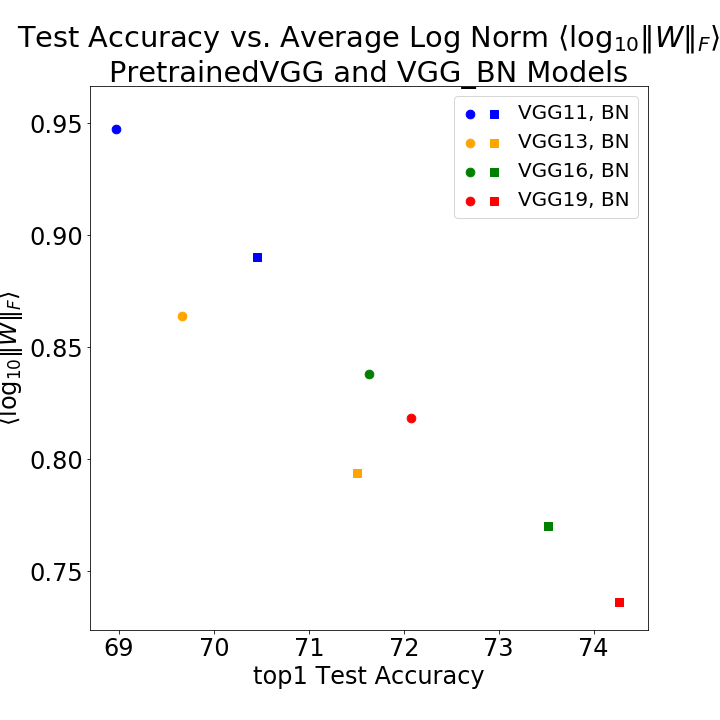
\includegraphics[scale=0.25]{img/vgg-lognorms.png}
      \label{fig:vgg_lognorms}
   }
   \subfigure[weighted average PL exponent $\hat{\alpha}$]{
      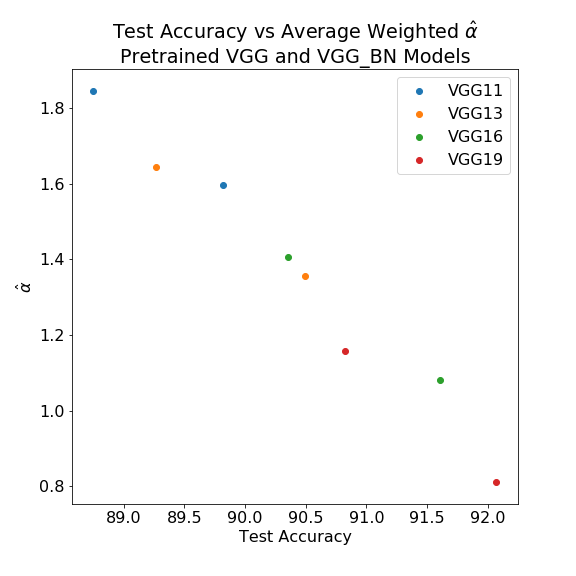
\includegraphics[scale=0.25]{img/vgg-w_alphas.png}
      \label{fig:vgg_alphahat}
   }
   \caption{%
      Pre-trained VGG and VGG\_BN Architectures and DNNs.  
      Top 1 Test Accuracy versus
      average log Frobenius norm $\langle\log\Vert\mathbf{W}\Vert_{F}\rangle$ (in (\ref{fig:vgg_lognorms}))
      or
      Universal, weighted average PL exponent $\hat{\alpha}$ (in (\ref{fig:vgg_alphahat}))
      for
      VGG11 vs VGG11\_BN ({\color{blue}{blue}}),
      VGG13 vs VGG13\_BN ({\color{orange}{orange}}),
      VGG16 vs VGG16\_BN ({\color{green}{green}}),  and
      VGG19 vs VGG19\_BN ({\color{red}{red}}). 
      We plot plain the VGG models with circles and the VGG\_BN models with~squares.
   }
   \label{fig:vgg}
\end{figure*}


%% COMBINED WITH ABOVE %% \begin{figure}[!htb]
%% COMBINED WITH ABOVE %%  \centering
%% COMBINED WITH ABOVE %%    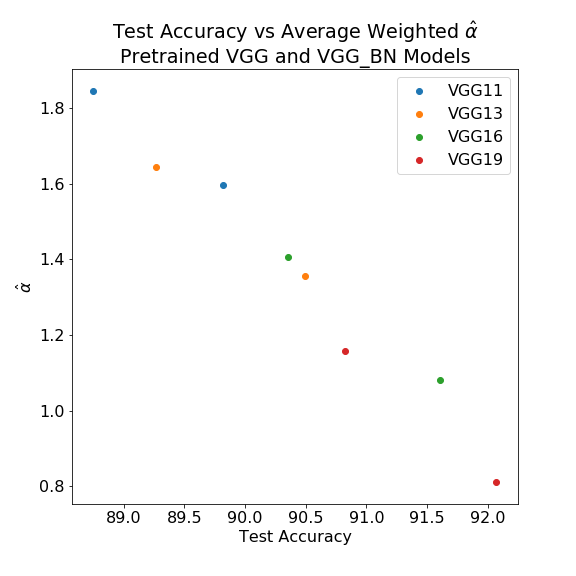
\includegraphics[scale=0.40]{img/vgg-w_alphas.png}
%% COMBINED WITH ABOVE %%    \caption{
%% COMBINED WITH ABOVE %% Pre-trained VGG and VGG BN Architectures and DNNs.  Test Accuracy and weighted average $\hat{\alpha}$ for
%% COMBINED WITH ABOVE %%  VGG11 vs VGG11\_BN ({\color{blue}{blue}}),
%% COMBINED WITH ABOVE %% VGG13 vs VGG13\_BN ({\color{orange}{orange}}),
%% COMBINED WITH ABOVE %% VGG16 vs VGG16\_BN ({\color{green}{green}}),  and
%% COMBINED WITH ABOVE %% VGG19 vs VGG19\_BN ({\color{red}{red}}). 
%% COMBINED WITH ABOVE %% }
%% COMBINED WITH ABOVE %%   \label{fig:vgg_alphahat}
%% COMBINED WITH ABOVE %% \end{figure}



\begin{table}[t]
\small
\begin{center}
\begin{tabular}{|p{0.75in}|c|c|c|c|c|c|c|}
\hline
Model & Top1 Accuracy & $\hat{\alpha}$ \\
\hline
VGG11 & 68.97 & 1.84 \\
VGG11\_BN & 70.45 & 1.60 \\
\hline
VGG13 & 69.66 & 1.65 \\
VGG13\_BN & 71.51 & 1.36 \\
\hline
VGG16 & 71.64 & 1.41 \\
VGG16\_BN & 73.52 & 1.08 \\
\hline
VGG19 & 72.08 & 1.16 \\
VGG19\_BN & 74.27 & 0.81 \\
\hline
\end{tabular}
\end{center}
\caption{%
         Results for VGG Architecture.   The Top1 Accuracy is defined
as the $100.0$ minus the Top1 reported error.
         }
\label{table:models_VGG}
\end{table}


We first look at the VGG class of models, comparing the log norm and the Universal $\hat{\alpha}$ metrics.
See Figure~\ref{fig:vgg} and Table~\ref{table:models_VGG} for a summary of the results.
Figures~\ref{fig:vgg_lognorms} and~\ref{fig:vgg_alphahat} show both the average log Frobenius norm, $\langle\log\Vert\mathbf{W}\Vert_{F}\rangle$ of Eqn.~(\ref{eqn:av_log_norm}), and the weighted average PL exponent, $\hat{\alpha}$ of Eqn.~(\ref{eqn:alpha_hat_specific}), as a function of the reported (Top1) test accuracy for the series of pre-trained VGG models, as available in the pyTorch package.%
\footnote{\url{https://pytorch.org/}}
These models include VGG11, VGG13, VGG16, and VGG19, as well as their more accurate counterparts with Batch Normalization, VGG11\_BN, VGG13\_BN, VGG16\_BN and VGG19\_BN. 
%See Figures~\ref{fig:vgg_lognorms} and~\ref{fig:vgg_alphahat} as well as Table~\ref{table:models_VGG} for details.
Table~\ref{table:models_VGG} provides additional details.

%Figure~\ref{fig:vgg_lognorms} shows the average log Frobenius norm results, which are quite good; and 
%Figure \ref{fig:vgg_alphahat} shows the weighted average PL exponent results, which yield slight improvements due to the method we introduce.
Across the entire series of architectures, 
reported test accuracies increase linearly as each metric, 
%%the average log Frobenius norm 
$\langle\log\Vert\mathbf{W}\Vert_{F}\rangle$
%%, Eqn.~(\ref{eqn:av_log_norm}), 
and 
%%the average weighted power law exponent 
$\hat{\alpha}$,
%%, Eqn.~(\ref{eqn}).
decreases.
Moreover, whereas the log norm relation has 2 outliers, VGG13 and VGG13\_BN, the Universal $\hat{\alpha}$ metric shows a near perfect linear relation across the entire VGG~series.

\paragraph{ResNet Models.}

\begin{figure*}[!htb]
   \centering
   \subfigure[log Frobenius norm $\langle\log\Vert\mathbf{W}\Vert_{F}\rangle$]{
      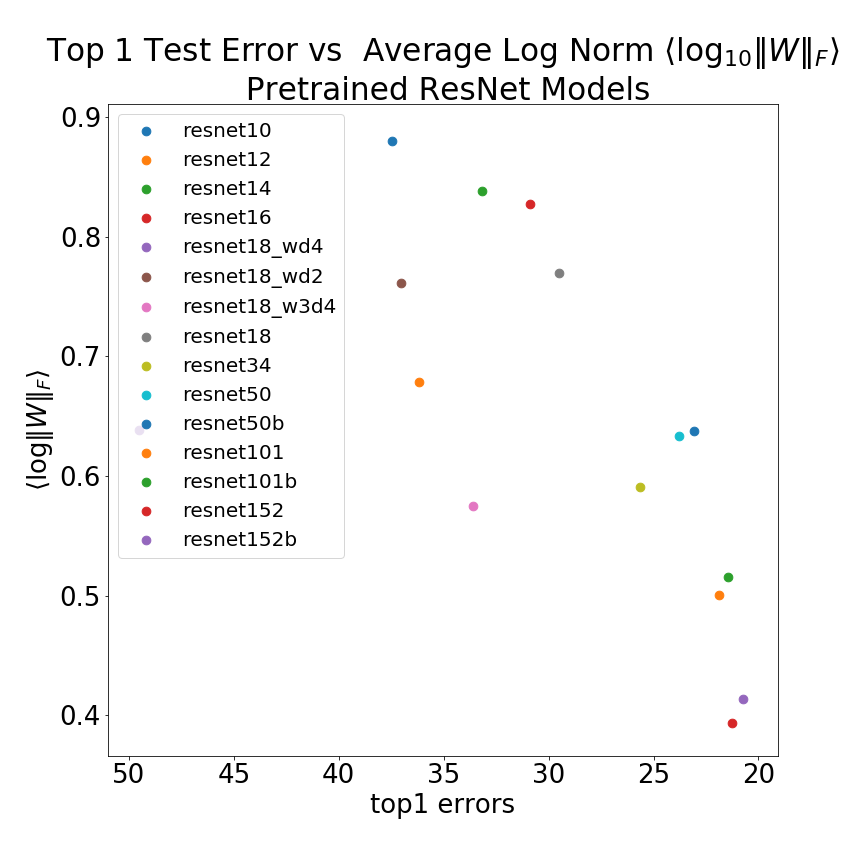
\includegraphics[scale=0.21]{img/ResNet_top1-lognorms.png}
      \label{fig:resnet_lognorms}
   }
   \subfigure[weighted average PL exponent $\hat{\alpha}$]{
      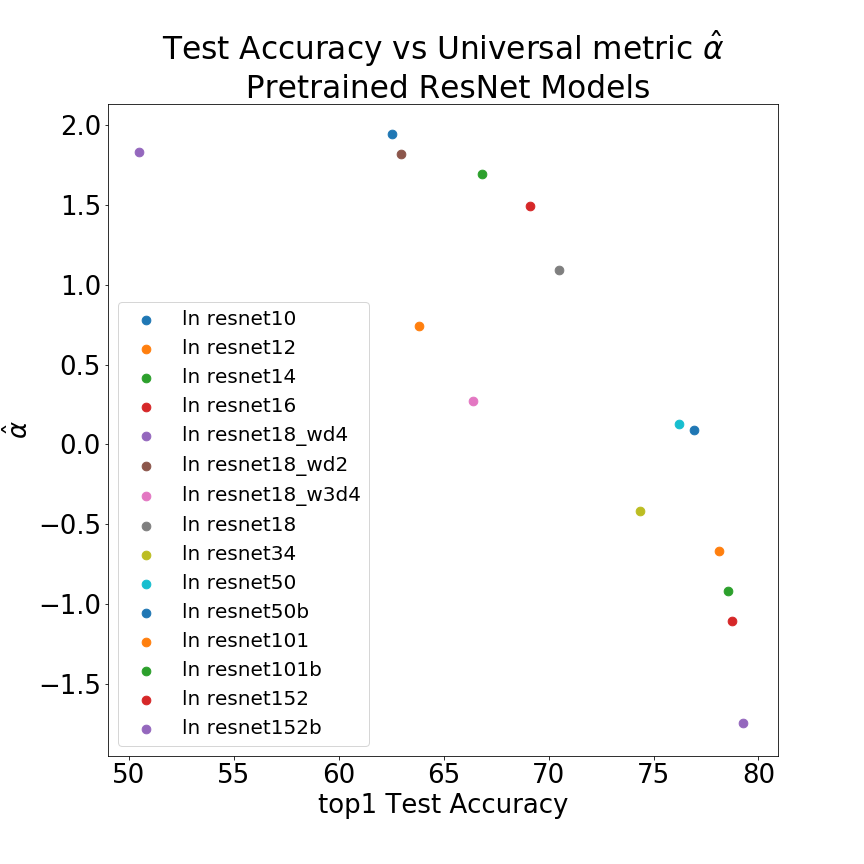
\includegraphics[scale=0.21]{img/ResNet-w_alphas.png}
      \label{fig:resnet_alphahat}
   }
   \caption{
      Pre-trained
      ResNet Architectures and DNNs.  
      Top 1 Test Accuracy versus
      average log Frobenius norm $\langle\log\Vert\mathbf{W}\Vert_{F}\rangle$ (in (\ref{fig:resnet_lognorms}))
      or
      Universal, weighted average PL exponent $\hat{\alpha}$ (in (\ref{fig:resnet_alphahat})).
           }
   \label{fig:resnet}
\end{figure*}

\begin{table}[t] %[!htb]
\small
\begin{center}
\begin{tabular}{|p{0.75in}|c|c|c|c|c|c|c|}
\hline
Architecture 
 & Model
 & Top 1 Accuracy & $\hat{\alpha}$ \\
\hline
ResNet (small)   & resnet10 & 62.54 & 1.94 \\
 & resnet12 & 63.82 & 0.74 \\
 & resnet14 & 66.83 & 1.70 \\
 & resnet16 & 69.10 & 1.49 \\
 \hline
 ResNet18  & resnet18\_wd4 & 50.50 & 1.83 \\
 & resnet18\_wd2 & 62.96 & 1.82 \\
 & resnet18\_w3d4 & 66.39 & 0.28 \\
 & resnet18 & 70.48 & 1.09 \\
 \hline
ResNet34 & resnet34 & 74.34 & -0.42 \\
\hline
ResNet50  & resnet50 & 76.21 & 0.13 \\
 & resnet50b & 76.95 & 0.09 \\
 \hline
ResNet101 & resnet101 & 78.10 & -0.67 \\
 & resnet101b & 78.55 & -0.92 \\
\hline
ResNet152 & resnet152 & 78.74 & -1.11 \\
 & resnet152b & 79.26 & -1.74 \\
\hline
\end{tabular}
\end{center}
\caption{Results for ResNet Architectures and DNN Models.  The Top1 Accuracy is defined
as the $100.0$ minus the Top1 reported error.  Some $\hat{\alpha}<0$ because the of how
the ResNet weight matrices are internally scale and normalized, which makes the maximum eigenvalue
less then one, $\lambda^{max}<1$.
        }
\label{table:models_resnet}
\end{table}

We next look at the ResNet class of models. 
See Figure~\ref{fig:resnet} and Table~\ref{table:models_resnet} for a summary of the results.
Here, we consider a set of 15 different pre-trained ResNet models, of varying sizes and accuracies, ranging from the small ResNet10 up to the largest ResNet152 models, as provided by the OSMR sandbox,%
\footnote{\url{https://github.com/osmr/imgclsmob}}
developed for training large-scale image classification networks for embedded systems.
Again, we compare the reported (Top1) test accuracy versus the average log norm $\langle\log\Vert\mathbf{W}\Vert_{F}\rangle$ and the Universal $\hat{\alpha}$ metrics. 

As with the VGG series, both metrics monotonically decrease as the test accuracies decrease for the ResNet series, and both metrics have a few large outliers off the main line relation. 
See Figures~\ref{fig:resnet_lognorms} and~\ref{fig:resnet_alphahat}.
In particular, the log norm metric has several notable outliers, including resnet18\_wd2, resnet18\_wd3\_d4, resnet34, and resnet10. 
The $\hat{\alpha}$ metric shows a slightly better relation, with resnet18\_wd2 more in line, and the other 3 outliers a little less off the main line of correlation. 
The Universal $\hat{\alpha}$ metric is as good or slightly better than the average log norm metric for the Resnet series of models. 

We see similar results for our Universal PL capacity control metric $\hat{\alpha}$ across a wide range of other pre-trained DNN models, described in Appendix~\ref{sxn:appendix-addl-empirical}.
In nearly all cases, the metric $\hat{\alpha}$ correlates well with the reported test accuracies, with only a three DNN architectures as exceptions. 
Overall the $\hat{\alpha}$ metric systematically correlates well with the generalization accuracy of a wide class of pre-trained DNN architectures---which is rather remarkable.


%\vspace{-4mm}
\section{Discussion and Conclusion}
\label{sxn:discussion}
%\vspace{-3mm}

We have presented an \emph{unsupervised} capacity control metric which predicts trends in test accuracies of a trained DNN---without peeking at the test data. 
In the interests of space, see Appendix~\ref{sxn:appendix-addl-discussion} for additional discussion.
We conclude by observing simply that 
%We expect our result will have applications in the fine-tuning of DNN hyperparameters as well as related challenges.
%Moreover, because we do not need to peek at the test data, our approach may prevent information from leaking from the test set into the model, thereby helping to prevent overtraining and making fined-tuned DNNs more robust.
%Finally, 
our work also leads to a much harder theoretical question: is it possible to characterize properties of realistic DNNs to determine whether a DNN is overtrained---without peeking at the test data?  




\bibliographystyle{unsrt}
%\bibliographystyle{plain}

{\small
%\bibliography{gen_gap}
%\bibliography{dnns}
\bibliography{dnns,gen_gap}
}

\appendix
%\newpage

%% \section{Appendix: Real DNN versus HT Random Matrices}
%% \label{sxn:appendix-dnn_versus_random}
%% 
%% \michael{MM still to fix this.}
%% 
%% \paragraph{Properties of our Basic Relation of Eqn.~(\ref{eqn:basic_relation}).}
%% XXX.  MAYBE PUT THIS IN APPENDIX.
%% 
%% \charlesX{
%% TODO:  explain plots.
%% Refer to Figure~\ref{fig:relations}.
%% 
%% Multiplying $\alpha$ by $\log_{10}\lambda_{max}$, we now have a relation that increases nearly linearly with the Frobenius norm for a random matrix, and is linearly correlated for real DNN data. Which is exactly what we want for our simple complexity metric.
%% 
%% Note that while linear relation holds over several log scales, 
%% the relation does deviate from linearity at the smaller values of $\alpha\;\log_{10}\;\lambda_{max}$.
%% This is readily explained below .  
%% XXX.  WHAT FIG ARE WE REFERRING TO, PRESUMABLY FIG~\ref{fig:relation-vgg11}.
%% }
%% 
%%  \begin{figure}[t] %[!htb]
%%     \centering
%%    \subfigure[Random Pareto Matrices] {
%%        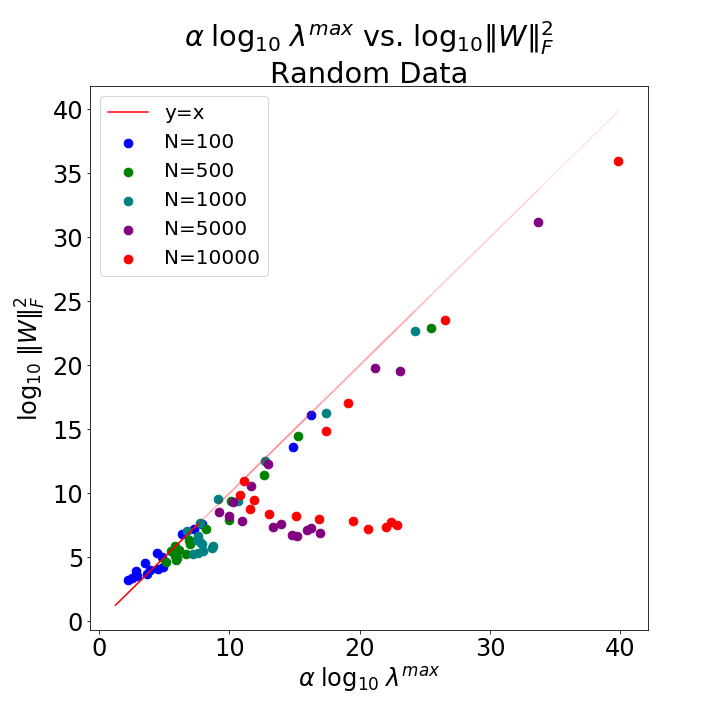
\includegraphics[scale=0.30]{img/relation-rand.png} 
%%        \label{fig:relation-rand}
%%    }
%%    \subfigure[VGG 11 Weight matrices]{
%%        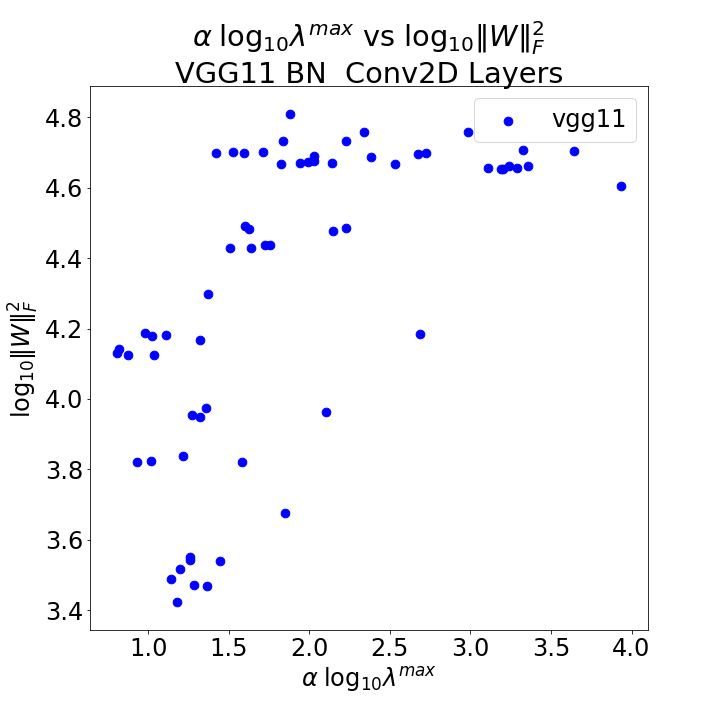
\includegraphics[scale=0.30]{img/relation-vgg11.png} 
%%        \label{fig:relation-vgg11}
%%    }
%%        \caption{Relation between $\alpha\;\log_{10}\;\lambda_{max}$ and the Frobenius norm squared }
%%    \label{fig:relations}
%%\end{figure}
%%
%%
%% \paragraph{Numerical Properties of Eqn.~(\ref{eqn:basic_relation}).}
%% 
%% We demonstrate that this relation holds numerically for both Heavy Tailed random matrices and for the weight matrices in pre-trained DNNs. 
%% 
%% XXX.  MOVE PROBABLY TO THE APPENDIX.
%% 
%% To understand this relation better, and to sketch a proof,
%% we will generate the data for a number of a Heavy-Tailed random matrices, 
%% with different power law exponents $\mu$.
%% And we compare defining correlation matrices $\mathbf{X}$, and therefore $\lambda_{max}$,
%% the Spectral norm (squared) of $\mathbf{W}$, with different normalizations.
%% 
%% \nred{Below} 
%% we generate a large number of  Heavy-Tailed  random matrices $\mathbf{W}^{rand}(\mu,M)$, with different number of eigenvalues $M$ (with aspect ratio $Q=1$), and drawn from a Pareto distribution,
%% $$
%% \Pr[{W}^{rand}_{i,j}]\sim\dfrac{1}{x^{1+\mu}}  ,
%% $$
%% with exponents $\mu\in[0.5, 5]$.
%% %
%% We then fit the ESD of each $\mathbf{W}^{rand}(\mu)$ to a PL using the method of Clauset et al.~\cite{CSN09_powerlaw,ABP14} to obtain the empirical exponent $\alpha$.  
%% 
%%MM%% \charles{describe, give pesudocode}.
%%MM%% 
%%MM%% For the Universality class of VHT ($1<\mu<2$), in order to form the limiting eigenvalue distribution $\rho_{\infty}(\lambda)$,
%%MM%% we require that the sum of any row of $\mathbf{W}$ converges as $N\rightarrow\infty$. This means a largest  element of any row
%%MM%% must be of order $\mathcal{O}(1)$.  By eqn (x) above, this implies that a typical element  (i.e the variance) scales as $\mathbf{W}^{0}\sim N^{-1/\mu}$, where $1<\mu<2$.
%%MM%% Of course, we do not known $\mu$, and most matrices are only moderately Heavy-Tailed, not very Heavy-Tailed.
%%MM%% Indeed, we are using RMT to model a strongly correlated system, so the scaling parameter
%%MM%% we have is the power law exponent $\alpha$ from our empirical fit.
%%MM%% Moreover, in a practical setting, we normalize $\mathbf{X}$ by $1/N$, but the empirical variance is not $1/N$, it is determined by the Frobenius norm squared
%%MM%% $\Vert\mathbf{W}\Vert^{2}_{F}$.   
%%MM%% 
%%MM%% We note that squared Frobenius norm is just the Trace of $\mathbf{W}^{T}\mathbf{W}$
%%MM%% \nred{which is just the sum of the Singular Values  $\sigma_{i}$ of $M$ squared:}
%%MM%% 
%%MM%% $$\Vert\mathbf{W}\Vert_{F}^{2}=\mbox{Trace}[\mathbf{W}^{T}\mathbf{W}]=\sum_{i=1}^{M}\sigma^{2}_{i}$$
%% 
%% If, however, we use the scale-dependent $1/N$ normalization to compute the correlations $\mathbf{X}$, we get very different behavior.
%% Figure~\ref{fig:randW} displays the same as above, as a function of the power law exponent \nred{(that was fit)}
%% $$
%% \dfrac{\log\Vert\mathbf{W}\Vert^{2}_{F}}{\log\lambda_{max}}\;\;vs.\;\;(\alpha)  .
%% $$
%% 
%% 
%% The numerical results for the the Power Law-Norm relation shows several interesting features: 
%% First, as $\alpha$ increases, we see the relation for
%% \begin{itemize}
%% \item  $\alpha<2$ , a near linear relation 
%% \item  $\alpha>2$ for $N,M$ large, the relation saturates, becoming constant
%% \item  $\alpha>2$  for smaller $N,M$,  a nearly linear relation, but with strong finite-size effects
%% \end{itemize}
%% These observations lead to a novel linear relation between the Frobenius norm and the power law exponent for our Heavy tailed matrices:
%% $$
%% \log\Vert\mathbf{W}\Vert^{2}_{F}\approx\alpha\log\lambda_{max}  ,
%% $$
%% which works very well for VHT Levy matrices, $\alpha<2$, and is a good approximation for MHT matrices and even some WHT matrices. 
%% And we believe this is the first time this relation has been noted in the literature.
%% 
%% 
%% \begin{figure}[t] %[!htb]
%%    \centering
%%    \subfigure[$\dfrac{1}{N}$ normalization] {
%%       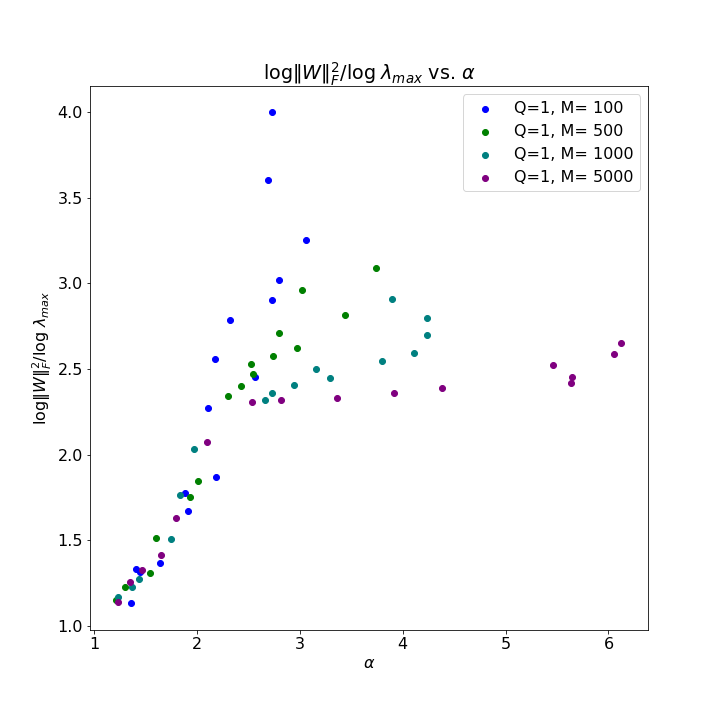
\includegraphics[scale=0.30]{img/Alpha-LogNorm-Relations.png}
%%       \label{fig:randW}
%%    }
%%    \subfigure[$\dfrac{1}{N^{2/\mu}}$ normalization] {
%%       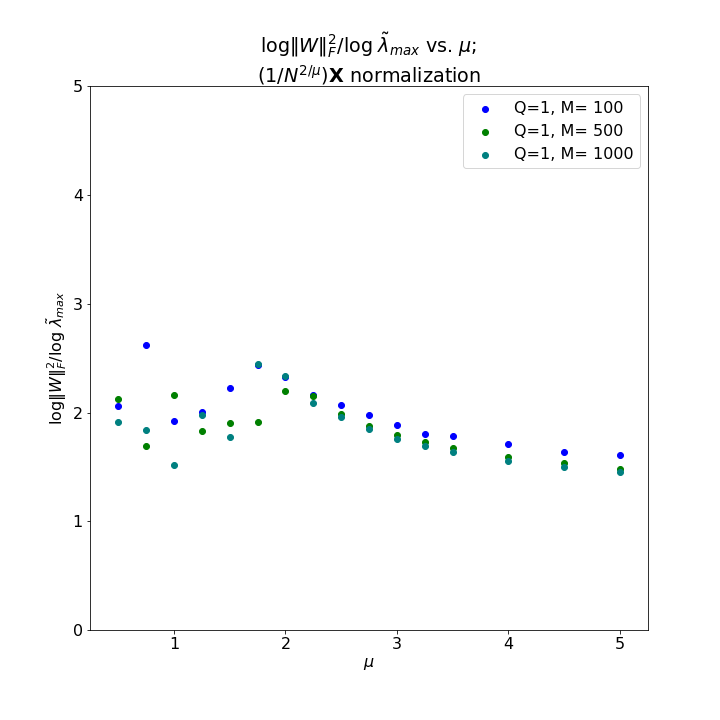
\includegraphics[scale=0.30]{img/LogNorm-Lmax-Scaled.png}
%%       \label{fig:logNormHat}
%%    }
%%    \caption{
%%             Numerical test of Eqn.~(\ref{eqn:basic_relation}) for random HT matrices; and the effect of different normalizations.
%%             \michael{Careful about $\alpha$ versus $\mu$ here.}
%%             \michael{Mention finite-size issues versus saturation.}
%%            }
%% \end{figure}
%% 
%% If, instead, we normalize the correlation matrix $\mathbf{X}$ by $N^{2/\mu}$, then we get very different behavior.
%% Let 
%% %$$
%% %\tilde{\mathbf{X}}=\dfrac{1}{N^{2/\mu}}\mathbf{W}^{T}\mathbf{W}  ,
%% %$$
%% $
%% \tilde{\mathbf{X}}=\dfrac{1}N^{-2/\mu}\mathbf{W}^{T}\mathbf{W}  ,
%% $
%% in which case we call $\tilde{\lambda}$ a \emph{scale-free eigenvalue} of $\tilde{\mathbf{X}}$, i.e.,
%% $  %$$
%% \tilde{\mathbf{X}}\mathbf{v}=\tilde{\mathbf{X}}\tilde{\lambda}  .
%% $  %$$
%% If we compute the scale-free eigenvalues, and we fit them to a PL exponent $\tilde{\alpha}$, then we find that the Frobenius norm is dominated by the maximum (scaled) eigenvalue $\tilde{\lambda}$ of $\tilde{\mathbf{X}}$.  
%% This is depicted in 
%% Figure~\ref{fig:logNormHat}
%% for our simulated Pareto matrices $\mathbf{W}^{rand}(\mu)$ which shows
%% %the log Frobenius norm squared, $\log_{10}\Vert\mathbf{W}\Vert^{2}_{F}$, divided by $\log_{10}\tilde{\lambda}$,
%% $\log\Vert\mathbf{W}\Vert^{2}_{F}/\log\tilde{\lambda}$,
%% for all for all ranges of $\mu$.
%% 
%% %%\begin{figure}[!htb]
%% %%   \centering
%% %%   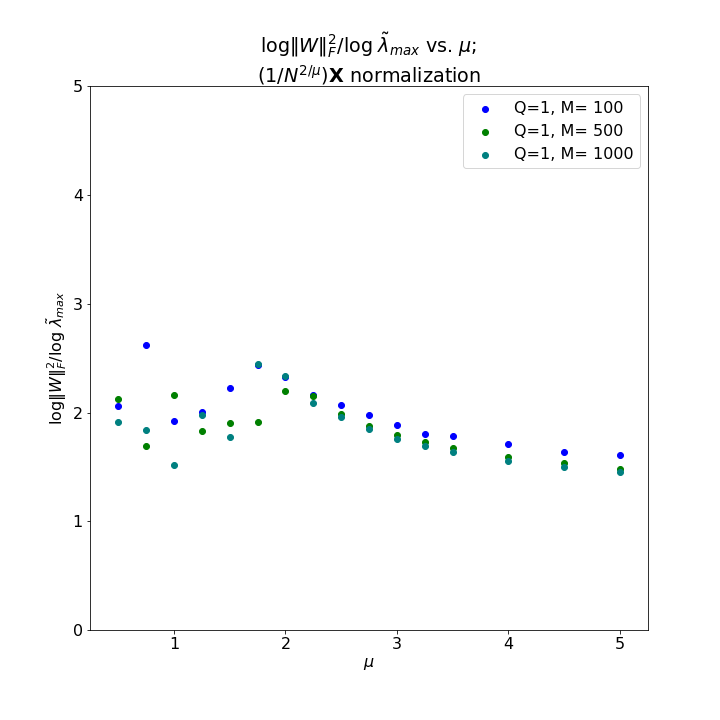
\includegraphics[scale=0.30]{img/LogNorm-Lmax-Scaled.png}
%% %%   \caption{R XXX.  WE MAY WANT THREE SUBFIGURES HERE.
%% %%   \michael{Charles suggest we don't need this figure and related discussion, decide later as text evolves.}
%% %%   }
%% %%  \label{fig:logNormHat}
%% %%\end{figure}
%% 
%% \charlesX{UGH I forgot why this is 2 .. we need to review the data and what was done and check the math carefully}\michael{Is this comment stale or still to deal with.}
%% 
%% Notice that this linear relations holds quite well, albeit with a large error bar, for $1<\mu<2$, even for small matrices, but starts to degrade for $\mu>2$.
%% This simple linear relation characterizes the scale invariant properties of the VHT Levy matrices; they are dominated by the largest scale-free eigenvalue.
%% 
%% $$\Vert\mathbf{W^{rand}(\mu)}\Vert^{2}_{F}\approx\tilde{\lambda}_{max},\;\;\mu=1$$
%% 
%% \nred{This might need to be
%% $$\Vert\mathbf{W^{rand}(\mu)}\Vert^{2}_{F}\approx\tilde{\sigma}^{2}_{max},\;\;\mu=1$$
%% }
%% 
%% which is good to within $5\%$ on a log scale
%% 
%% $$\log\;\Vert\mathbf{W^{rand}(\mu)}\Vert^{2}_{F}\approx\log\;\tilde{\lambda}_{max},\;\;1<\mu<2$$


\section{Random Pareto versus Non-random DNN Matrices} 
%\section{Heavy-Tailed Universality: Random Pareto versus Non-random DNN Matrices} 
\label{sxn:appendix-universality}

When we use Universality, as we do in our derivation of the basic PL--Norm Relation, we would like a method that applies both to HT random matrices as well as to non-random, indeed strongly-correlated, pre-trained DNN layer weight matrices that (as evidenced by their ESD properties) are in a HT Universality class.  
To accomplish this, however, requires some care: while the pre-trained $\mathbf{W}$ matrices do have ESDs that display empirical signatures of HT Universality~\cite{MM18_TR}, they are \emph{not} random Pareto matrices.
Many of their properties, including their empirical Frobenius norms, behave very differently than that of a random Pareto matrix.  
(We saw this in Figure~\ref{fig:relations}, which showed that $ \alpha\log\lambda_{max} $ achieves much larger values for HT random matrices than real DNN weight matrices.)

To illustrate this, we generate a large number of HT random matrices $\mathbf{W}^{rand}(\mu)$, with exponents $\mu\in[0.5, 5]$, as described in Section~\ref{sxn:theory-new}.
%
We then fit the ESD of each $\mathbf{W}^{rand}(\mu)$ to a PL using the method of Clauset et al.~\cite{CSN09_powerlaw,ABP14} to obtain the empirical exponent $\alpha$. 
Figure~\ref{fig:fro-rand} displays the relationship between the (log of the squared) Frobenius norm and the $\mu$ exponents for these randomly-generated Pareto matrices.
(Similar but noisier plots would arise if we plotted as a function of $\alpha$, due to imperfections in the PL fit.)
We did the same for the weight matrices (extracted from the Conv2D Feature Maps) from the pre-trained VGG11 DNN, again as described in Section~\ref{sxn:theory-new}.
Figure~\ref{fig:fro-vgg11} displays these results, here as a function of $\alpha$.
\michael{Charles, maybe plot both as a function of $\alpha$, since they are different, and consistent with text.}

\begin{figure}[!htb]
   \centering
   \subfigure[Random Pareto Matrices] {
      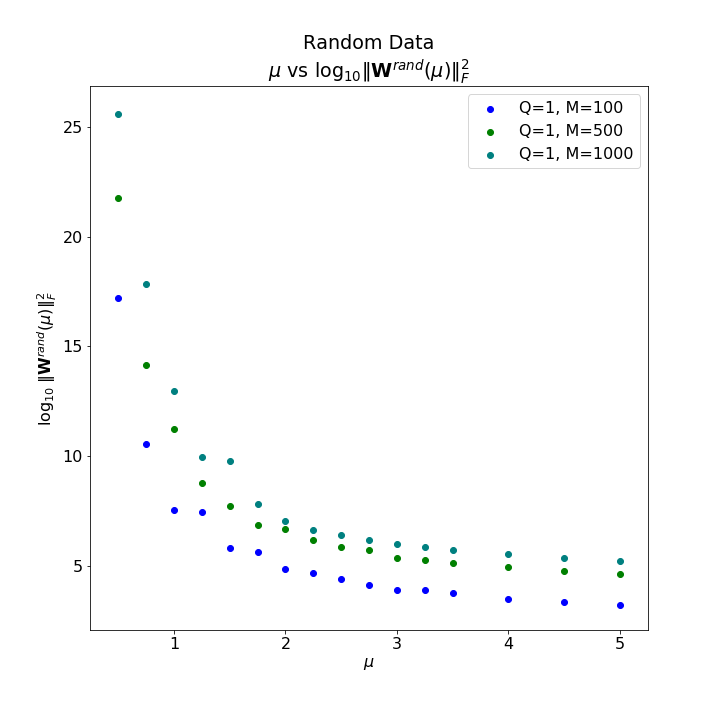
\includegraphics[scale=0.30]{img/fro-rand.png} 
      \label{fig:fro-rand}
   }
   \subfigure[Pre-trained VGG11 Weight Matrices]{
      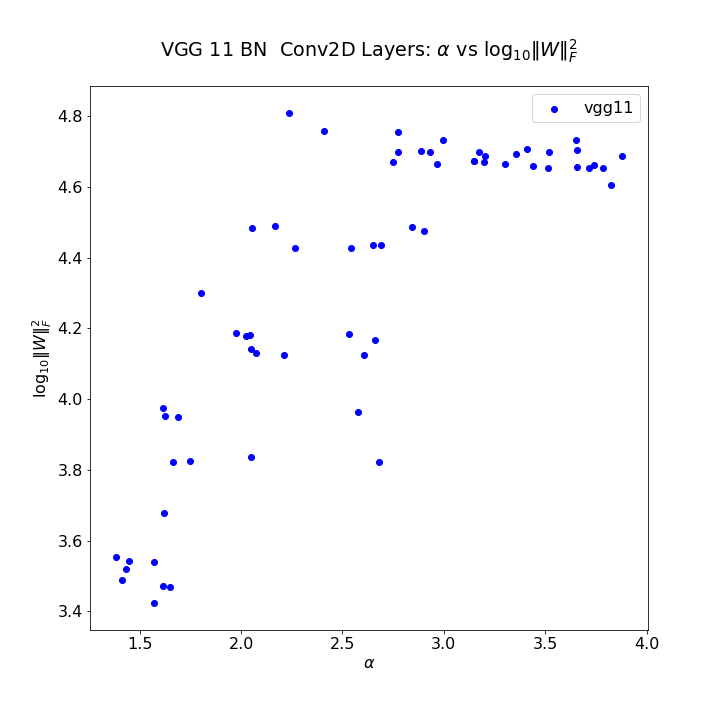
\includegraphics[scale=0.30]{img/fro-vgg11.png} 
      \label{fig:fro-vgg11}
   }
   \caption{Dependence of Frobenius norm on PL exponents for random Pareto versus pre-trained DNN matrices.  }
   \label{fig:fnorm}
\end{figure}

The properties of $\Vert\mathbf{W}\Vert^{2}_{F}$ for the random Pareto versus real/ron-random DNN weight matrices are quite different.
For a random Pareto matrix, $\mathbf{W}^{rand}(\mu)$, the Frobenius norm $\Vert\mathbf{W}^{rand}(\mu)\Vert^{2}_{F}$ 
\emph{decreases with increasing exponent} $(\mu)$; and there is a modest finite-size effect.
(In addition, as the tails of the ESD $\rho(\lambda)$ get heavier, the largest eigenvalue $\lambda_{max}$ of $\mathbf{X}$ scales with the largest element of $\mathbf{W}^{rand}(\mu)$.) 
% \michael{$\alpha$ or $\mu$ here.}
% \michael{Cite something or show this.}
For the weight matrices of a pre-trained DNN, however, the Frobenius norm $\Vert\mathbf{W}\Vert^{2}_{F}$ \emph{increases with increasing exponent} $(\alpha)$, saturating at $\alpha\approx 3$.
This happens because, due to the training process, the $\mathbf{W}$ matrices themselves are highly-correlated, and not random matrices with a single large, atypical element.
In spite of this, the ESD $\rho(\lambda)$ of these pre-trained correlations matrices $\mathbf{X}$ display Universal HT behavior~\cite{MM18_TR}; and, as shown in Figure~\ref{fig:relation-vgg11}, 
Eqn.~(\ref{eqn:basic_relation}) is approximately satisfied, in the sense that 
$\alpha\log\lambda_{max}$ is positively correlated with $\log\Vert\mathbf{W}\Vert^{2}_{F} $.
This is one of the remarkable properties of Universality (and it shows why some care must be taken in applying these Universality principles).
 

\newpage
\section{Appendix: Michael's Derivation}
\label{sxn:appendix-michael_derivation}

\michael{MM probably remove this entirely, unless relate to synthetic empirical results.}

Here, we derive an expression for the ratio of the log of the Frobenius norm of $W$ to the log of the spectral norm of $W$.
Once we settle on presentation, with normaliation, etc., this will probably be a ``subroutine'' in our analysis.
To simplify things, we will be interested in the matrix $W$, and in particular the Frobenius norm $\|W\|_F$ and spectral norm $\|W\|_2$ of this matrix.
Then, given these expressions, we will derive other things, e.g., norms of correlation matrices with different normalizations, etc., by using different normalizations.  

Recall that we are modeling the matrix $W$ as a random matrix with heavy-tailed entries.
XXX.  WE MIGHT WANT A FIGURE SHOWING THE REAL DATA LOOKS LIKE THIS, LIKE THE BURDA PAPER.
Thus, the Frobenius norm is going to be related to the second moment of the entries, and the spectral norm is going to be related to the largest entry.
XXX.  CITE AUFFINGER PAPER FOR EXACTLY THE RANGE OF VALIDITY OF THIS.
An important issue will be the power law exponent, since---depending on it---familiar results will hold or will fail to hold.
For the moment, let's ignore that we are dealing with matrices, and let's focus on drawing elements from a heavy-tailed distribution, and computing various moments and extreme values of empirical draws.

Consider the extreme case of a HT distribution, namely a PL distribution.
XXX.  INCLUDE SOMETHING ABOUT SLOWLY VARYING FUNCTION AS WELL AS XMIN VALUE.
Up to a slowly-varying function, the general form of the probability distribution function is
$$
p(x) = \frac{C}{x^{1+\mu}}  = C x^{-1-\mu} , 
$$
where $\mu > -1$, and where $x \in [x_{min},\infty)$.
The cdf 
XXX ACTUALLY ONE MINUS THAT 
is then
$$
P_{\ge}(x) = \int_x^{\infty} p(x^{\prime}) dx^{\prime} 
           = \frac{C}{\mu} \frac{1}{x^{\mu}}  
           = \frac{C}{\mu} x^{-\mu}  .
$$
In order to compute $C$ and normalize these expressions, let
\begin{eqnarray*}
1 = \int_{x_{min}}^{\infty} p(x) dx 
  = C \int_{x_{min}}^{\infty} x^{-1-\mu} dx 
  = \frac{C}{-\mu} x^{-\mu} |_{x_{min}}^{\infty}  
  = \frac{C}{\mu} x_{min}^{-\mu}   ,
\end{eqnarray*}
which is valid (i.e., the integral converges and exists) if $\mu > 0$.
From this, is follows that the normalization constant is
\begin{equation}
C = \mu x_{min}^{\mu}  .
\label{eqn:pl_normalization}
\end{equation}
Thus, if $\mu > 0$, then the probability distribution function is 
\begin{equation}
p(x) 
%     = \frac{\mu}{x_{min}}\left( \frac{x_{min}}{x}\right)^{1+\mu}  
     = \frac{\mu}{x_{min}}\left( \frac{x}{x_{min}}\right)^{-1-\mu}  ,
\label{eqn:pl_pdf}
\end{equation}
and the cdf 
XXX ACTUALLY ONE MINUS THAT
is 
\begin{equation}
P_{\ge}(x) 
%           = \left( \frac{x_{min}}{x} \right)^{\mu}  
           = \left( \frac{x}{x_{min}} \right)^{-\mu}  .
\label{eqn:pl_one_minus_cdf}
\end{equation}
XXX.  MENTION SLOWLY VARYING THING, MAYBE AS CLAUSET DID.

An important aspect of heavy-tailed probability distributions is that extreme values, i.e., values very far from the mean (when the mean is even defined) are not extremely uncommon (as they are for distributions in the Gaussian universality class).
Of particular relevance for us is the largest value $x_{max}$ obtained when sampling from Eqn.~(\ref{eqn:pl_pdf}) in $n$ i.i.d. trials.
It is known, see e.g.~\cite{SornetteBook,BouchaudPotters03,newman2005_zipf}, that the expectation of $x_{max}$ for $\mu\in(1,2)$ 
XXX IS THIS TRUE FOR MORE GENERAL PL PARAMETERS
is given~by:
$$
\ExpectBracket{x_{max}} \approx x_{min} n^{1/\mu}  .
$$

Let's return to the expression given in Eqn.~(\ref{eqn:pl_pdf}) and compute the first few moments of this distribution.
The first moment is
\begin{eqnarray*}
\ExpectBracket{x} = \int_{x_{min}}^{\infty} x p(x) dx  
                  = C \int_{x_{min}}^{\infty} x^{-\mu} dx 
                  = \frac{C}{1-\mu} x^{1-\mu} |_{x_{min}}^{\infty} 
                  = \frac{\mu}{\mu-1} x_{min}    ,
\end{eqnarray*}
which is valid if $\mu > 1$.
Similarly, the second moment is
\begin{eqnarray*}
\ExpectBracket{x^2} = \int_{x_{min}}^{\infty} x^2 p(x) dx  
                    = C \int_{x_{min}}^{\infty} x^{1-\mu} dx 
                    = \frac{C}{2-\mu} x^{2-\mu} |_{x_{min}}^{\infty} 
                    = \frac{\mu}{\mu-2} x_{min}^2  ,  
\end{eqnarray*}
which is valid if $\mu > 2$.
While this second moment expression is valid for $\mu > 2$, we are going to want a similar expression for $\mu \in (1,2)$.
For this we can integrate up to $x_{max}$, rather than up to $\infty$.
In more detail, for $\mu \in (1,2)$, the empirical second moment is
\begin{eqnarray*}
\ExpectBracket{x^2} &=&       \int_{x_{min}}^{x_{max}} x^2 p(x) dx  \\
                    &=&       \frac{C}{2-\mu} x^{2-\mu} |_{x_{min}}^{x_{max}}  \\
                    &\approx& \frac{\mu}{2-\mu} x_{min}^{\mu} \left( x_{min}^{2-\mu} n^{(2-\mu)/\mu} - x_{min}^{2-\mu} \right) \\
                    &\approx& \frac{\mu}{2-\mu} x_{min}^{2} n^{(2-\mu)/\mu}   ,
\end{eqnarray*}
which is valid for $\mu\in(1,2)$.
Note that in these expressions and the expressions below, we follow previous work \cite{MM18_TR} and don't compute expressions for $\mu=2$ precisely.
(They are known to lie in yet another universality class~\cite{SornetteBook,BouchaudPotters03}, and we don't expect to resolve the difference numerically.)

Finally, consider an $N \times N$ matrix $W$. 
Then, 
$\|W\|_2 = w_{min} N^{2/\mu}$ (for $\mu\in(1,2)$) and
$\|W\|_2 = w_{min} N^{1/2}$ (for $\mu>2$).
XXX.  CHECK THAT I AM NOT OFF By A FACTOR OF N.
Thus, for the spectral norm, we have that: 
\begin{equation}
\|W\|_2^2 = \left\{ \begin{array}{ll}
                       w_{min}^2 N^{4/\mu} & \mbox{if $\mu\in(1,2)$} \\
                       w_{min}^2 N & \mbox{if $\mu > 2$} (XXX CHECK)
                    \end{array}
            \right.
\end{equation}
Similarly, for the Frobenius norm, we have that:
\begin{equation}
\|W\|_F^2 = \left\{ \begin{array}{ll}
                      \frac{\mu}{2-\mu} w_{min}^2 N^{(4-2\mu)/\mu} & \mbox{if $\mu\in(1,2)$} \\
                      \frac{\mu}{\mu-2} w_{min}^2 N^2 & \mbox{if $\mu > 2$} 
                    \end{array}
            \right.
\end{equation}

We are interested in the function of $\mu$ defined as:
$$
f = f(\mu) = \frac{\log \|W\|_F^2}{\log \|W\|_2^2}  .
$$
From the above, if we take logs, then for $\mu\in(1,0)$, we get:
$$
f(\mu) = \frac{ \log\left(\frac{\mu}{2-\mu}\right) + \log(w_{min}^2) + \frac{4}{\mu}\log N - 2 \log N }{ \log(w_{min}^2) + \frac{4}{\mu}\log N }
$$
and for $\mu > 2$, we get:
$$
f(\mu) = \frac{ \log\left(\frac{\mu}{\mu-2}\right) + \log(w_{min}^2) + 2 \log N }{ \log(w_{min}^2) + \log N }
$$


% \section{Appendix: Refs: MM TO INCORPORATE THESE INTO TEXT}
% 
% Our theory of Implicit Self Regularization used Heavy Tailed Random Matrix Theory (HT RMT), and here we use HT RMT also~\cite{MM18_TR}.
% See also our prior results on \cite{MM17_TR}.
% 
% \cite{NTS14_TR} is 
% Neyshabur et al. on :
% ``In search of the real inductive bias: on the role of implicit regularization in deep learning''
% 
% \cite{NTS15} is
% Neyshabur et al. on:
% ``Norm-Based Capacity Control in Neural Network''
% 
% \cite{NBMS17_TR} is 
% Neyshabur et al. on:
% ``Exploring generalization in deep learning''
% 
% \cite{AGNZ18_TR} is 
% Arora et al. on:
% ``Stronger generalization bounds for deep nets via a compression approach''
% 
% \cite{ACH18_TR} is 
% Arora et al. on:
% ``On the Optimization of Deep Networks: Implicit Acceleration by Overparameterization''
% 
% \cite{Bar97} is
% Bartlett on:
% ``For valid generalization, the size of the weights is more important than the size of the network''
% 
% \cite{BFT17_TR} is 
% Bartlett et al. on:
% ``Spectrally-normalized margin bounds for neural networks''
% 
% \cite{SHNx17_TR} is 
% Soudry et al. on: 
% ``The implicit bias of gradient descent on separable data''
% 
% \cite{YM17_TR} is 
% Yoshida and Miyato on:
% ``Spectral norm regularization for improving the generalizability of deep learning''
% 
% \cite{LMBx18_TR} is 
% Liao et al. on:
% ``A surprising linear relationship predicts test performance in deep networks''
% 
% \cite{PLMx18_TR}
% is Poggio el at. on: 
% ``Theory {IIIb}: Generalization in Deep Networks''
% 
% \cite{KKB17_TR} is 
% Kawaguchi et al. on:
% ``Generalization in Deep Learning''
% 
% \cite{NBS17_TR} is:
% Neyshabur et al. on: 
% ``A {PAC}-{B}ayesian Approach to Spectrally-Normalized Margin Bounds for Neural Networks''
% 
% \cite{ZF18_TR} is
% Zhou and Feng on:
% ``Understanding Generalization and Optimization Performance of Deep {CNN}s''
% 
% \cite{BJNx01_TR} is
% Burda et al. on:
% ``{L}{\'e}vy Matrices and Financial Covariances''
% 
% \cite{MN09_TR} is
% Mahoney and Narayanan on:
% ``Learning with Spectral Kernels and Heavy-Tailed Data''
 




\end{document}


